\documentclass[11pt,a4paper]{article}
\usepackage[top=3cm, bottom=2cm, left=2cm, right=2cm]{geometry}
\usepackage[utf8]{inputenc}
\usepackage{amsmath, amsfonts, amssymb}
\usepackage{siunitx}
\usepackage[brazil]{babel}
\usepackage{graphicx}
\usepackage[margin=10pt,font={small, it},labelfont=bf, textfont=it]{caption}
\usepackage[dvipsnames, svgnames]{xcolor}
\DeclareCaptionFont{MediumOrchid}{\color[svgnames]{MediumOrchid}}
\usepackage[pdftex]{hyperref}
\usepackage{natbib}
\bibliographystyle{plainnat}
\bibpunct{[}{]}{,}{s}{}{}
\usepackage{color}
\usepackage{footnote}
\usepackage{setspace}
\usepackage{booktabs}
\usepackage{multirow}
\usepackage{subfigure}
\usepackage{fancyhdr}
\usepackage{leading}
\usepackage{indentfirst}
\usepackage{wrapfig}
\usepackage{mdframed}
\usepackage{etoolbox}
\usepackage[version=4]{mhchem}
\usepackage{enumitem}
\usepackage{caption}
\usepackage{titlesec}
\usepackage{tcolorbox}
\usepackage{tikz}
\usepackage{LobsterTwo}
\usepackage[T1]{fontenc}
\usepackage{fontspec}
\usepackage{txfonts}
\AtBeginEnvironment{equation}{\fontsize{13}{16}\selectfont}


\titleformat{\section}{\LobsterTwo\LARGE\color{CarnationPink}}{\thesection.}{1em}{}
\titleformat{\subsection}{\LobsterTwo\LARGE\color{CarnationPink}}{\thesubsection}{1em}{}


\DeclareCaptionLabelFormat{figuras}{\textcolor{DarkTurquoise}{Figura \arabic{figure}}}
\captionsetup[figure]{labelformat=figuras}

\makeatletter
\renewcommand\tagform@[1]{\maketag@@@{\color{CarnationPink}(#1)}}
\makeatother

\renewcommand{\theequation}{Eq. \arabic{equation}}
\renewcommand{\thefigure}{Fig. \arabic{figure}}
\renewcommand{\thesection}{\textcolor{CarnationPink}{\arabic{section}}}

\setlist[itemize]{label=\textcolor{CarnationPink}{$\mathbf{\square}$}}

\setlist[enumerate]{label=\textcolor{CarnationPink}{\arabic*.}, align=left}


\newcounter{exemplo}

\NewDocumentEnvironment{exemplo}{ O{} }{%
\allowbreak
\setlength{\parindent}{0pt}
  \begin{mdframed}[
  leftline=true,
  topline=false,
  rightline=false,
  bottomline=false,
  linewidth=2pt,
  linecolor=CarnationPink,
  frametitlerule=false,
  frametitlefont=\LobsterTwo\large\color{CarnationPink},
  frametitle={\color{CarnationPink}\LobsterTwo\large #1},
  ]
}{%
  \end{mdframed}
}

\setlength{\fboxsep}{5pt}
\setlength{\fboxrule}{1.5pt}
\usepackage{float}
\renewcommand{\thefootnote}{\alph{footnote}}
\usepackage{url}
\hypersetup{
	colorlinks=true,
	linkcolor=DarkTurquoise,
	filecolor=DarkTurquoise,      
	urlcolor=DarkTurquoise,
	citecolor=DarkTurquoise,
	pdftitle={Especialista em Física da Radioterapia}
}
\pagestyle{fancy}
\fancyhf{}
\renewcommand{\headrulewidth}{0pt}
\rfoot{Página \thepage}

\title{\LobsterTwo\Huge{Garantia Da Qualidade}}
\author{\LobsterTwo\Large{QA em Cálculos de Dose}\nocite{*}}
\date{\LobsterTwo\textit{Dalila Mendonça}}
\begin{document}
	\maketitle

\section{Introdução}

    Um componente-chave da radioterapia segura e eficaz é a capacidade de alinhar precisamente um paciente em relação ao campo de radiação durante o tratamento. Os meios atuais de conseguir isso incluem a visualização 3D de estruturas de tecidos moles (via tomografia computadorizada (TC) ou ultrassom e, agora,  ressonância magnética (MRI)), localização 2D ou 3D de pontos de referência ósseos ou fiduciais (imagens planares de kV/MV ou rastreamento de marcadores implantados) e alinhamento de substitutos, como um ``bite block'' ou marcadores reflexivos. O uso mais extensivo dessas técnicas é para radioterapia guiada por imagem (IGRT), que regularmente usa imagens (às vezes diariamente), geralmente com uma modalidade volumétrica. 

\section{Sistemas de Imagens}

    A tecnologia e o uso de sistemas de imagem durante o tratamento continuam a evoluir em ritmo acelerado. Vários artigos foram publicados sobre este tema e a maior parte dos relatórios de consenso tentam fornecer visões gerais, das quais o documento AAPM TG-104, \textit{The Role of In-Room kV X-Ray Imaging for Patient Setup and Target Localization} é notável por sua perspectiva histórica que remonta ao uso de fontes kV acopladas a Unidades de tratamento \ce{^{60}Co} no final dos anos 1950. Atualmente, as tecnologias mais usadas incluem as seguintes (listas em AAPM TG-104/AAPM TG-179):

    \begin{itemize}[label=\textcolor{CarnationPink}{$\blacktriangleright$}]
        \item  CT de feixe cônico de quilovoltagem (kV-CBCT), por exemplo:
        \begin{itemize}[label=\textcolor{CarnationPink}{$\star$}]
            \item sistema On-Board Imaging (OBI) (Varian Inc., Palo Alto, CA);
            \item Sistema Synergy X-ray Volume Imager (XVI) (Elekta, Inc., Crawley, Reino Unido).
            \item  Dispositivo de imagem de painel plano em modo fluoroscópico; 2 imagens de projeção por grau com faixa de rotação do gantry de \ang{200} a \ang{360}; Aquisição de 1 a 2 minutos. Essas unidades também são capazes de realizar radiografias e fluoroscopia.
        \end{itemize}
        
        \item Imagens planares de megavoltagem (imagens de portal) usadas em sistemas baseados em gantry. Documentos de referência: AAPM TG-58 (cerca de 2001) e padrões CAPC QC para EPIDs. Foi desenvolvido tecnicas para utilizar imagens de MV para verificar a administração da dose imediatamente antes do tratamento ou durante o próprio tratamento, uma abordagem conhecida como dosimetria EPID in vivo.
        
        \item Fan-beam MV-CT (TomoTherapy/Accuray, Madison, WI). CT usando o feixe de 3.5 MeV, feixe colimado de 4 mm com pitch 1 a 3 (AAPM TG-148).
        
        \item In-room CT on rails (``TC na sala sobre trilhos''). Menos amplamente utilizado do que as tecnologias acima, embora imagens de qualidade diagnóstica estejam disponíveis. 
        
        \item Imagem kV estereoscópica planar. Utilizam câmaras de imagem de tubo de raios X/ painéis planos emparelhados montados no chão e no teto para determinar mudanças relativas à DRRs. Os sistemas kV de energia dupla estão se tornando comercialmente disponíveis, que permitem imagens de subtração para melhorar a visualização dos tecidos moles. Exemplos:
        \begin{itemize}[label=\textcolor{CarnationPink}{$\star$}]
            \item Sistema CyberKnife (Accuray Inc., Sunnyvale, CA);
            \item Sistema Novalis ExacTrac (BrainLab AG, Feldkirchen, Alemanha).
        \end{itemize}
        
        \item “Sistemas combinados” (ou seja, estereoscópico planar mais kV-CBCT). Exemplos:
        \begin{itemize}[label=\textcolor{CarnationPink}{$\star$}]
            \item NovalisTx platform (Varian Inc., Palo Alto, CA);
            \item  Vero (Mitsubishi Heavy Industries, Ltd. \& Brainlab AG), usando o acelerador MHI-TM2000 e um par de tubos de raios X/painéis de imagens planos montados em um conjunto de O-ring giratório.
        \end{itemize}

        \item Tomossíntese digital. Situada em algum lugar entre a imagem planar e a TC, essa técnica renderiza um “plano espesso” perpendicular ao feixe, adquirindo imagens em uma pequena faixa de ângulos ($<$ \ang{40}).
    \end{itemize}

    Além dos sistemas acima, várias tecnologias “complementares” estão disponíveis para localização durante o tratamento:
    
    \begin{itemize}[label=\textcolor{CarnationPink}{$\blacktriangleright$}]
        \item  O ultrassom tem sido usado para localizar a próstata e a cavidade cirúrgica na mama durante o tratamento. Um sistema de câmera estabelece a relação geométrica entre a sonda transdutora da ultrassom e o isocentro de tratamento. Os produtos comerciais incluem SonArray (Varian Medical Systems, Palo Alto, CA) e Clarity (Elekta Inc., Crawley, Reino Unido). Os desafios incluem variabilidade inter-usuário (e a importância associada do treinamento do usuário), pressão abdominal (foram observados deslocamentos de 5 mm) e movimento intra-fração (um estudo observou deslocamentos de 5 mm em 3\% do tempo).

        \item Vários sistemas de localização estão disponíveis e dependem de imagens da superfície do paciente e/ou marcadores superficiais (isto é, sistemas de localização não radiográficos). Uma classe de sistemas usa duas ou mais câmeras estereoscópicas para criar imagens de marcadores reflexivos infravermelhos. Estes incluem o sistema FreeTrack (Varian Medical Systems, Palo Alto, CA), que alinha um bite block para tratamentos intracranianos; ExacTrac (BrainLab AG, Feldkirchen, Alemanha); DynaTrac (Elekta Inc., Crawley, Reino Unido); e CyberKnife (Accuray Inc., Sunnyvale, CA), todos os quais usam marcadores reflexivos em alguns modos de operação.
        
        \item Outros sistemas dependem da projeção de padrões de luz estruturados na superfície do paciente (por exemplo, AlignRT, VisionRT Ltd., Londres, Reino Unido) ou lasers projetados (Sentinel, C-Rad, Uppsala, Suécia). Uma limitação fundamental de todos esses sistemas é a dependência de recursos na superfície de um paciente, que podem não se correlacionar com a posição da anatomia interna de interesse.
        
        \item Uma classe de localização não radiográfica depende de transponders eletromagnéticos implantados cuja localização pode ser determinada por meio de uma bobina fonte/receptor na superfície do paciente ou próximo a ela. Um sistema, Calypso (comercializado pela Varian Medical Systems, Palo Alto, CA) usa dispositivos transponder implantados de 8 mm x 2 mm. Na próstata, três beacons ``guias'' são tipicamente implantados a partir dos quais a rotação/translação da glândula pode ser determinada.
        
        \item Imagens de RM em MR-60Co treatment unit (ViewRay Inc., Bedford, OH) e Aceleradores lineares acoplados a MR.
        
    \end{itemize}

    Os centros de radioterapia de prótons também empregam orientação por imagem durante o tratamento, que é brevemente descrita na AAPM TG-104. Quase todos os centros de radioterapia de prótons atualmente dependem de radiografia planar kV e não utilizam TC durante o tratamento. 
    

\section{Imagem Radiográfica: Qualidade da Imagem e Dose}

    O desempenho da qualidade de imagem dos sistemas radiográficos é comumente caracterizado por cinco parâmetros:

    \begin{enumerate}
        \item Precisão geométrica;
        \item Resolução espacial;
        \item Resolução em baixo contraste;
        \item Ruído; e
        \item Uniformidade
    \end{enumerate}

    Uma discussão particularmente útil sobre contraste e ruído em imagens planares pode ser encontrada no AAPM TG-58, enquanto muitos relatórios discutem imagens de TC (por exemplo, AAPM TG-66, AAPM TG-104 e AAPM TG-179). Recentemente, foi proposto que um sistema possa ser desenvolvido para prever a técnica de imagem ideal para visualizar a detecção de características durante o IGRT.

    Para sistemas de TC durante o tratamento, o AAPM TG-179 cita o seguinte desempenho típico (Deve-se notar, porém, que a qualidade da imagem é altamente dependente da técnica.):

    \begin{enumerate}[label=\textcolor{CarnationPink}{\roman*.}]
        \item Precisão geométrica $<$ 1 mm;
        \item Resolução espacial de 6 a 9 pares de linhas/cm em imagens KV-CBCT ou 1.6 mm em objeto de alto contraste para MV-CBCT;
        \item Resolução de contraste de 1\% para um objeto de 7 mm em kV-CBCT e 2\% para um objeto de 13 mm em imagens de MC-CBCT.
    \end{enumerate}

    A qualidade da imagem da TC também é afetada por fatores relacionados ao paciente. Os implantes metálicos causam artefatos na TC devido ao endurecimento do feixe, o que pode obscurecer a visualização do tecido e afetar os cálculos dosimétricos se não forem tratados adequadamente. Exemplos de tais implantes são hardware ortopédico (suporte espinhal, hastes no úmero ou fêmur, próteses de quadril e semelhantes), obturações dentárias e marcadores fiduciais implantados.

    Artefatos são mais proeminentes em kV-CT (versus MV-CT) porque a imagem kV é mais afetada pela interação fotoelétrica, que tem um alto coeficiente de absorção em materiais de alto número atômico. Às vezes, o contraste intravenoso ou oral é usado para visualizar vasos ou esôfago/intestino. Isso também pode resultar em artefatos e afetar os cálculos de dose. 
    
    Outro artefato relacionado ao paciente é o ruído devido à privação de fótons e endurecimento do feixe. Isso pode ser especialmente evidenciado em pacientes grandes, embora o ruído possa ser reduzido nesses casos aumentando o kVp do tubo de raios X. Se alguma parte da anatomia do paciente estiver fora da região de reconstrução da TC, podem aparecer efeitos de borda (ou seja, “anéis” brilhantes na borda externa da imagem da TC).

    A qualidade da imagem em kV-CBCT merece consideração especial. A geometria de feixe cônico produz mais espalhamento do que um feixe de leque, resultando em aumento de ruído, redução de contraste e redução de uniformidade (em particular, artefato “cupping”). Quando os tamanhos dos pacientes são diferentes daqueles usados para calibração, números de TC incorretos podem ser retornados (AAPM TG-179 Seção IV.D). Esta é uma consideração importante se as aquisições do CBCT forem utilizadas para o cálculo da dose. Da mesma forma, os efeitos de imagem devem ser considerados ao usar imagens MV do TomoTherapy para planejamento.

    O kV-CBCT também está sujeito a outros artefatos de imagem, incluindo borramento devido ao movimento do paciente, streaks devido ao movimento de bolha de gás, artefatos de anel de pixels com resposta insuficiente no detector de imagem e artefatos de streaks devido a um número incompleto de projeção de imagens. Exemplos de artefatos de imagem podem ser encontrados na AAPM TG-104 Figura III-B-1.

\subsection*{Considerações Sobre a Dose}

    O AAPM TG-75 fornece uma consideração abrangente da dose devido a imagens radiográficas durante o tratamento. AAPM TG-75 e outros relatórios citam valores aproximados para a dose devido a imagem que estão listados na \ref{fig:doseEstimadasParaImagens}. Ao considerar esses números, deve-se reconhecer que a dose de imagem depende fortemente dos dispositivos, técnicas e do local que está sendo radiografado.

    \begin{figure}[h]
        \centering
        \fcolorbox{DarkTurquoise}{white}{%
            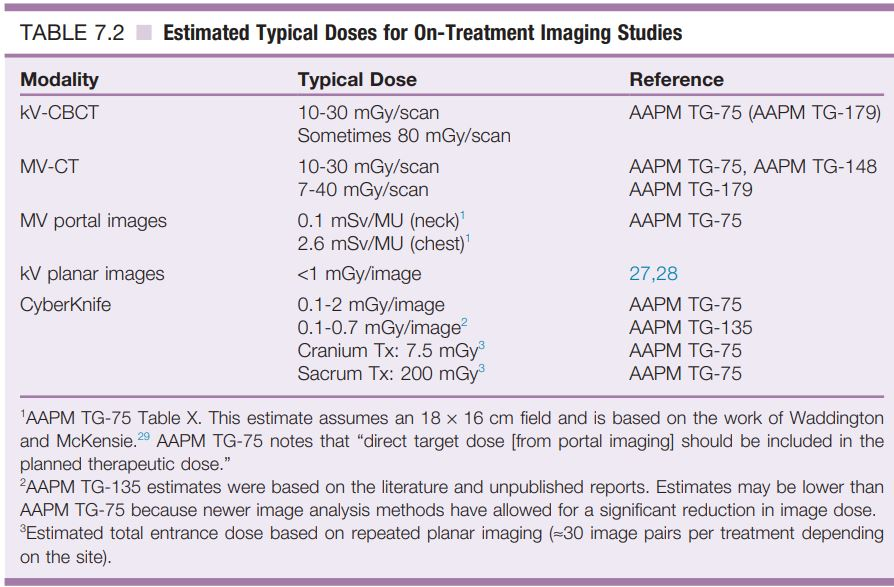
\includegraphics[width=0.8\textwidth]{Imagens/doseEstimadasParaImagens.JPG}
        }%
        \caption{Estimativa de dose para técnicas de IGRT}
        \label{fig:doseEstimadasParaImagens}
    \end{figure}

    A maioria dos valores na \ref{fig:doseEstimadasParaImagens} pode parecer pequenos, mas deve ser lembrado que o paciente recebe uma dose para todo o volume que está sendo examinado. Também, como contexto adicional, a dose entregue na imagem pode exceder a dose de fuga do acelerador linear (linac) em 1 ordem de grandeza, conforme apontado no AAPM TG-75. Além disso, a dose no osso pode ser aproximadamente três vezes maior que as doses listadas na \ref{fig:doseEstimadasParaImagens} devido ao efeito fotoelétrico. Portanto, vale a pena considerar a dose entregue pela imagem. Recomenda-se que a dose seja discutida com o Radio-oncologista de uma perspectiva clínica de custo/benefício. Isso é especialmente verdadeiro para pacientes pediátricos, que apresentam alto risco de malignidade secundária.
    
    O AAPM TG-75 discute maneiras de limitar a dose efetiva, em particular, restringindo a extensão superior/inferior da varredura ao mínimo necessário. A AAPM TG-75 recomenda que a dose de imagem seja incluída na dose terapêutica planejada, pelo menos no contexto da imagem portal MV.

    Existem alguns aspectos técnicos para medir e relatar a dose de TC que devem ser considerados. AAPM TG-75 e outros relatórios defendem o report da dose de CT em unidades de índice de dose de CT (CTDI). AAPM TG-66 Apêndice II fornece definições concisas desta e de grandezas relacionadas (ver também AAPM TG-75 Seção II.C.1, que apresenta material similar, mas com alguns erros nas definições). Parâmetros importantes são:

    \begin{itemize}[label=\textcolor{CarnationPink}{$\blacksquare$}]
        \item \textcolor{DarkTurquoise}{\textbf{$CTDI_{100}$:}} a dose medida em uma rotação de varredura em um comprimento longitudinal de 100 mm;
        \item \textcolor{DarkTurquoise}{\textbf{$CTDI_{w}$:}} a média ponderada das medidas de $CTDI_{100}$ em dois locais em um phantom especifico (um central e um periférico);
        \item \textcolor{DarkTurquoise}{\textbf{$CTDI_{vol}$:}} o “volume CTDI”, que inclui o efeito do pitch de varredura e é definido como $CTDI_{w}$/pitch. Valores típicos para $CTDI_{vol}$ e DLP em cerca de 2000 varreduras de TC kV de feixe em leque  são fornecidos na Tabela VII da AAPM TG-75, reunida a partir de dados extensos de centros europeus (10 a 80 mGy).
        \item \textcolor{DarkTurquoise}{\textbf{$DLP$:}} Produto do comprimento da dose, definido como $CTDI_{vol}$ multiplicado pelo comprimento da varredura;
    \end{itemize}

    Existem desafios com o uso de $CTDI_{100}$ em uma geometria de feixe cônico com mais de 100 mm porque a dose total não é medida como mostra a discussão no  \textit{``Human Health Report Num 5 on dosimetry in CBCT''} da Agência Internacional de Energia Atômica (IAEA) sobre dosimetria em CBCT. Finalmente, em termos de impacto para os pacientes, a quantidade mais relevante não é a dose absorvida, mas sim a dose efetiva (ponderada pelo órgão). Existem, no entanto, muitos desafios na estimativa da dose efetiva para TC durante o tratamento. A Seção IV da AAPM TG-75 descreve a metodologia para cálculos de dose efetiva e os desafios relacionados. Relatórios de dose medida dos sistemas de tratamento são frequentemente citados simplesmente em unidades de mGy (por exemplo, AAPM TG-75).

    \begin{tcolorbox}[width=\textwidth, colback={white}, colbacktitle={DarkTurquoise!50!white}, title={$\bigstar$ \LobsterTwo{Pitch} $\bigstar $}, coltitle={CarnationPink}, colframe={DarkTurquoise}, fonttitle=\rmfamily\bfseries\Large]
        Em uma tomografia computadorizada (TC), o termo "pitch" refere-se a uma medida que descreve o avanço da mesa durante o exame em relação à espessura do corte realizado pelo feixe de raios X. É uma medida importante que afeta a velocidade e a qualidade da aquisição das imagens na TC.

        \

        O pitch é calculado dividindo-se o avanço da mesa pelo valor da espessura do corte. Por exemplo, se a mesa se move 1 cm por rotação completa e o corte possui uma espessura de 0,5 cm, o pitch seria 2 (1 cm / 0,5 cm = 2). Quanto maior o valor do pitch, maior é o avanço da mesa em relação à espessura do corte.

        \

        O pitch afeta diretamente o tempo de aquisição das imagens na TC. Um pitch maior resulta em uma varredura mais rápida, pois a mesa avança mais durante cada rotação do tubo de raios X. No entanto, um pitch maior também pode levar a uma menor sobreposição das imagens, o que pode resultar em menor resolução espacial e possíveis artefatos na imagem. Por outro lado, um pitch menor resulta em uma varredura mais lenta, mas com maior sobreposição das imagens, o que geralmente resulta em uma melhor resolução espacial.
    \end{tcolorbox}

\section{Controle de Qualidade para Sistemas de Imagens}

    O teste de aceite e o comissionamento são os primeiros passos no controle de qualidade dos dispositivos de imagem e consistem principalmente na coleta de dados de desempenho para formar o baseline com os quais os futuros testes de controle de qualidade serão comparados. Durante o teste de aceite e comissionamento, os principais recursos do sistema precisam ser avaliados, incluindo funcionalidade, recursos de segurança, calibração e integração do sistema, incluindo a conectividade com o sistema de planejamento de tratamento (por exemplo, transferência de imagens de referência e contornos para o sistema IGRT). Testes adicionais incluem calibração geométrica, teste de posicionamento/reposicionamento e testes de qualidade de imagem. Todos os modos de operação e configurações devem ser considerados durante o teste de aceite e comissionamento. Vários relatórios da ASTRO e da ACR recomendam especificamente o uso de testes de localização end-to-end no momento do comissionamento ou em atualizações.

\subsection*{Controle de Qualidade Contínuo}

    Uma variedade de testes contínuos de controle de qualidade são necessários para garantir uma operação segura e de alta qualidade. A \ref{fig:qaImagensParte1} e a \ref{fig:qaImagensParte2} fornece uma visão geral dos testes de controle de qualidade padrão. Uma característica imediatamente óbvia na \ref{fig:qaImagensParte1} e na \ref{fig:qaImagensParte2} é a discordância entre os relatórios quanto à frequência e tolerância dos testes.

    \begin{figure}[!h]
        \centering
        \fcolorbox{DarkTurquoise}{white}{%
            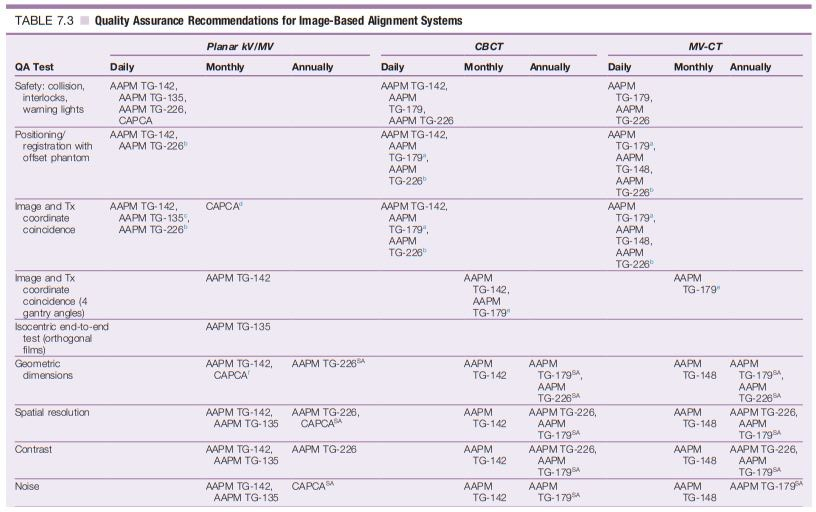
\includegraphics[width=0.8\textwidth]{Imagens/qaImagensParte1.JPG}
        }%
        \caption{QAs recomendados para sistemas de alinhamento baseados em imagens parte 1.}
        \label{fig:qaImagensParte1}
    \end{figure}

    \begin{figure}[!h]
        \centering
        \fcolorbox{DarkTurquoise}{white}{%
            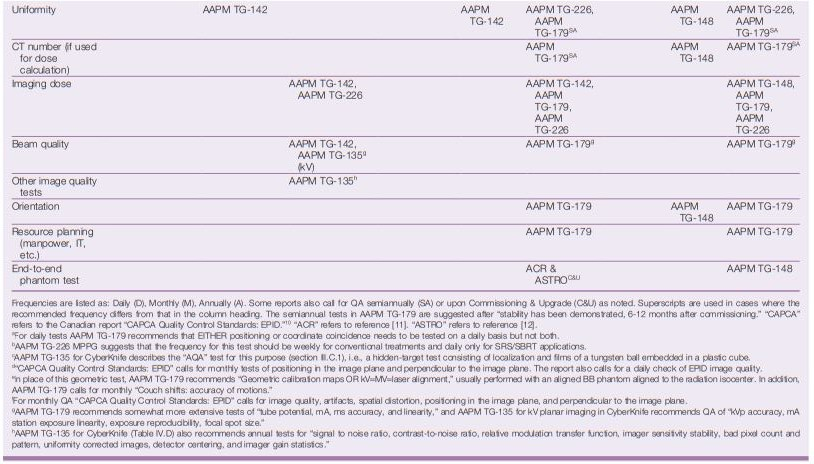
\includegraphics[width=0.8\textwidth]{Imagens/qaImagensParte2.JPG}
        }%
        \caption{QAs recomendados para sistemas de alinhamento baseados em imagens parte 2.}
        \label{fig:qaImagensParte2}
    \end{figure}

    Um aspecto do controle de qualidade que não é explicitamente observado nos dados apresentados na \ref{fig:qaImagensParte1} e na \ref{fig:qaImagensParte2} é a necessidade de controle de qualidade após grandes atualizações, reparos ou manutenção. A maioria dos relatórios exige esse controle de qualidade. Por exemplo, o AAPM TG-226 recomenda que o físico médico verifique ou restabeleça os baselines do controle de qualidade após atualização, reparo ou serviço. A \ref{fig:qaImagensParte1} e a \ref{fig:qaImagensParte2} apresentam as recomendações específicas mais importantes, mas não lista todos os recursos relacionados ao controle de qualidade. Outros documentos incluem o relatório ACR-ASTRO sobre IGRT e o \textit{``ASTRO safety white paper on IGRT''}.

    
    
    
\subsection*{QA Geométrico}

    A \ref{fig:qaImagensParte1} e  lista diversas variedades de testes geométricos de controle de qualidade. Um teste é para dimensionamento geométrico e normalmente emprega um objeto de tamanho conhecido para avaliar as dimensões geométricas geradas pelo sistema de imagem. Isso deverá testar todas as três dimensões, e a frequência recomendada é mensal (ou semestral, dependendo do report). 
    
    Alguns reports sugerem um teste anual de orientação geométrica dos sistemas de TC para garantir que a orientação correta da imagem seja retornada nas três dimensões cardeais. Isso normalmente é feito usando um phantom com vários marcadores. 
    
    Um teste geométrico final avalia o alinhamento entre o isocentro da imagem e o isocentro tratamento. Isso é particularmente importante em sistemas nos quais um sistema mecânico diferente é empregado para geração de imagens versus tratamento, como qualquer um dos atuais sistemas de geração de imagens baseados em kV. 

    A \ref{fig:pentaguide} mostra um exemplo de dispositivo para testes de alinhamento de imagens geométricas em sistemas utilizados em linacs. O cubo de plástico contém cavidades e/ou marcadores radiopacos que podem ser visualizados em uma imagem CBCT, bem como imagens planares de kV e MV. Isso fornece um teste diário rápido da coincidência de coordenadas de imagem e tratamento. Recomendações semelhantes podem ser encontradas no AAPM TG-148 para equipamentos TomoTherapy. Testes diários de posicionamento/reposicionamento também podem ser realizados com um dispositivo como o mostrado na \ref{fig:pentaguide}. 
    
    \begin{figure}[h]
        \centering
        \fcolorbox{DarkTurquoise}{white}{%
            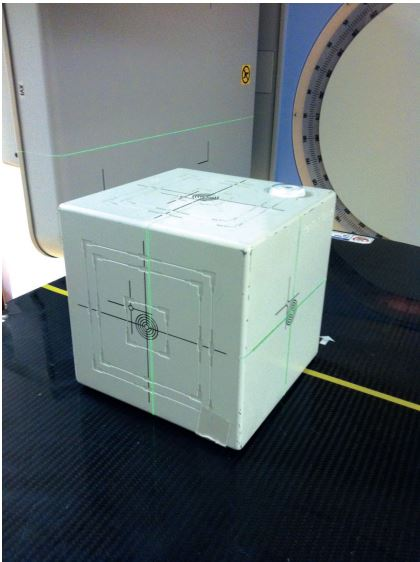
\includegraphics[width=0.5\textwidth]{Imagens/pentaguide.JPG}
        }%
        \caption{PentaGuide para alinhamento dos isocentros da Imagem e do linac.}
        \label{fig:pentaguide}
    \end{figure}
    

    O cubo de plástico é alinhado com o conjunto de marcadores no canto superior esquerdo. Uma tomografia computadorizada é então realizada e os fiduciais incorporados são alinhados a uma imagem de referência. A mesa do acelerador linear é deslocada pelo valor deslocamento de alinhamento medido. Se a imagem e o alinhamento estiverem corretos, o conjunto de marcas no centro do cubo (o “alvo”) será alinhado com os lasers no isocentro. O AAPM TG-142 e o AAPM TG-226 exigem esse teste diariamente, enquanto o AAPM TG-179 exige “deslocamentos de mesa: precisão dos movimentos” mensais. A AAPM TG-179 sugere que os desvios sejam $<$2 cm e desiguais em todos os eixos para descobrir possíveis erros.

    Mensalmente, “testes de alinhamento geométrico” mais extensos são indicados em alguns relatórios (por exemplo, AAPM TG-179, mas não AAPM TG-226). Descrições destes testes para CBCT podem ser encontradas com algum detalhe no AAPM TG-104 (Seção II.B.4), em visão geral no AAPM TG-179 (Seção IV.A). Resumidamente, este teste consiste em alinhar um “rolamento de esferas - ball bearing (BB)” com o isocentro MV, adquirindo imagens do portal em quatro ângulos cardeais do gantry (ângulos opostos do colimador também são adquiridos para eliminar o efeito de possível assimetria do jaw). A etapa alinha precisamente o BB com o isocentro de radiação e o desacopla de qualquer possível desalinhamento com os lasers. Essa etapa de alinhamento do BB ao isocentro da radiação é semelhante à usada em um teste de Winston-Lutz.

    Depois que o BB estiver alinhado, ele poderá ser usado para adquirir “flexmaps” se o sistema CT precisar ser recalibrado. De acordo com a AAPM TG-179, a recalibração geométrica deve ser realizada conforme recomendado pelo fabricante após grandes atualizações de hardware ou software ou após manutenção que possa afetar o sistema CT. Se a recalibração não for necessária, uma TC pode ser adquirida e o alinhamento geométrico pode ser medido como a distância do centro do BB ao centro do volume de TC reconstruído. O AAPM TG-148 recomenda que o alinhamento entre os sistemas de coordenadas de tratamento e imagem seja testado anualmente usando um phantom end-to-end com filme embutido, arranjos de diodos ou outros meios de medir a distribuição de dose administrada.

\subsection*{QA da Qualidade da Imagem}

    A \ref{fig:qaImagensParte2} fornecem uma visão geral dos testes recomendados de qualidade de imagem. Vários dispositivos comerciais estão disponíveis para este fim. Para QAs de qualidade de imagem planar MV, os fornecedores dos aceleradores lineares normalmente fornecem o phantom de Las Vegas (\ref{fig:lasVegasPhantom}). Este phantom é insuficiente, entretanto, no entanto é útil para realizar os testes de resolução e geometria descritos na \ref{fig:qaImagensParte1}.

    \begin{figure}[h]
        \centering
        \subfigure{
		\fcolorbox{DarkTurquoise}{white}{%
			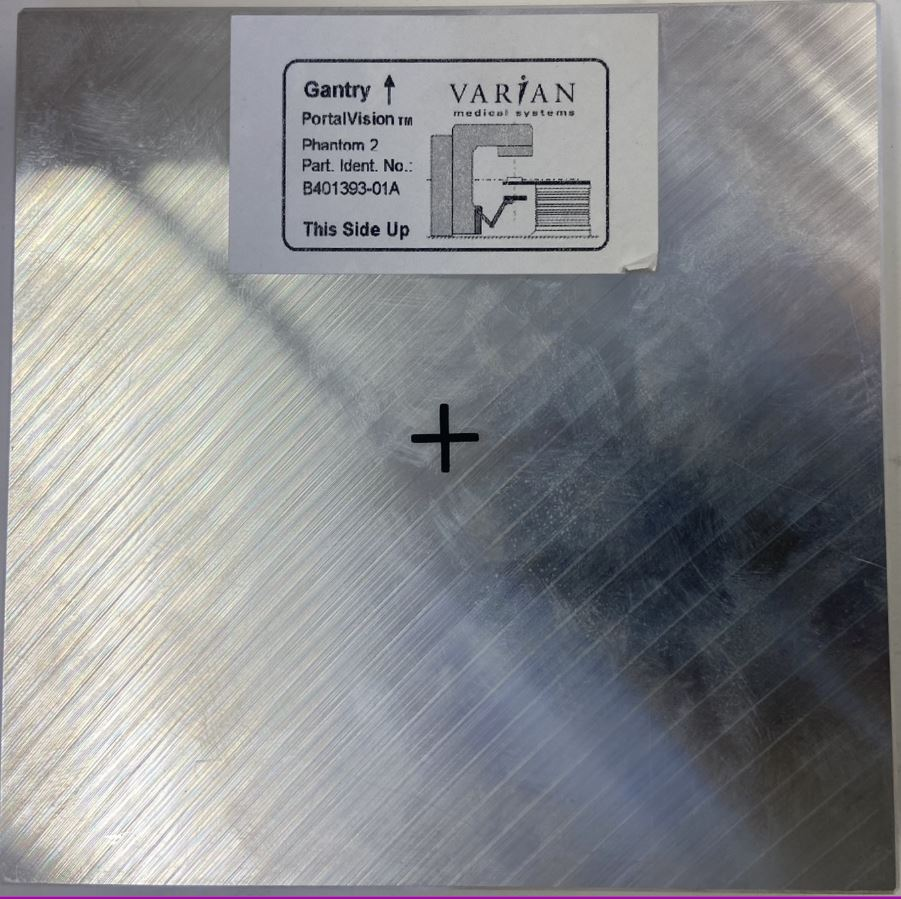
\includegraphics[width=0.4\textwidth]{Imagens/lasVegasPhantom1.JPG}
		}}%
        \subfigure{
		\fcolorbox{DarkTurquoise}{white}{%
			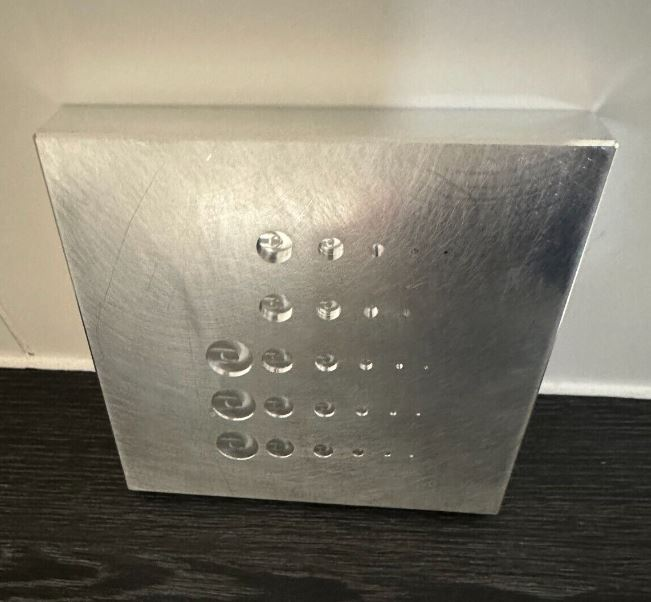
\includegraphics[width=0.43\textwidth]{Imagens/lasVegasPhantom.jpg}
		}} %
        \caption{Phantom Las Vegas fornecido pela Varian}
        \label{fig:lasVegasPhantom}
    \end{figure}

    A \ref{fig:qaImagemPlanarMV} mostra um dispositivo alternativo (QC-3 Phantom, Standard Imaging, Middleton, WI) para QA de imagens planares MV. A resolução espacial é medida com os objetos de pares de linhas embutidos na linha do meio, enquanto o contraste é medido com os quadrados e números ao longo de cada borda. Existe um dispositivo semelhante para o QA da qualidade de imagem planar kV. Os fornecedores geralmente fornecem o phantom Leeds TOR 18FG para essa finalidade (\ref{fig:torleeds}).

    \begin{figure}[h]
        \centering
        \subfigure{
		    \fcolorbox{DarkTurquoise}{white}{%
			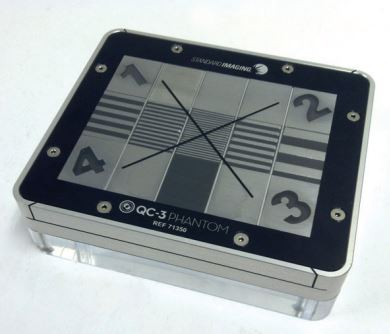
\includegraphics[width=0.44\textwidth]{Imagens/qaImagemPlanar.JPG}
		}}%
        \subfigure{
		    \fcolorbox{DarkTurquoise}{white}{%
			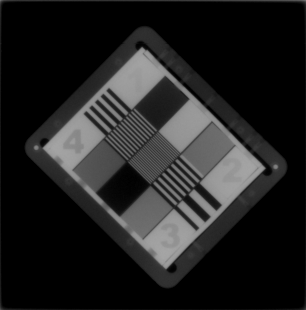
\includegraphics[width=0.37\textwidth]{Imagens/mceclip0.png}
		}}%
        \caption{QC-3 Phantom para QA de imagens planares MV}
        \label{fig:qaImagemPlanarMV}
    \end{figure}

    \begin{figure}[h]
        \centering
        \fcolorbox{DarkTurquoise}{white}{%
            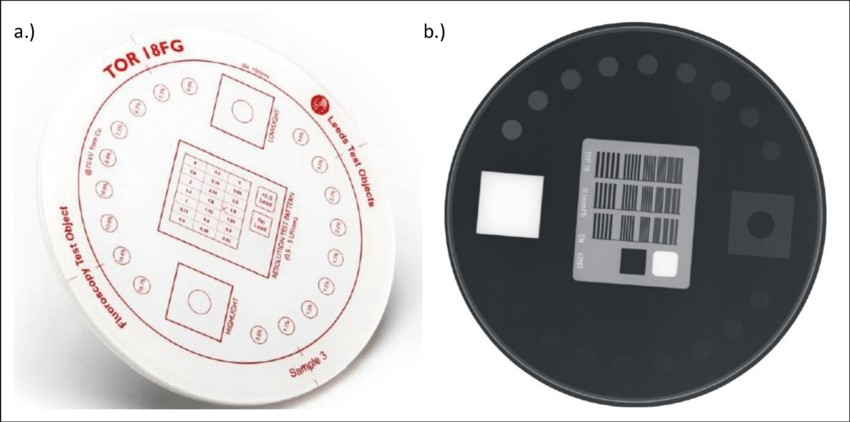
\includegraphics[width=0.8\textwidth]{Imagens/torleeds.jpg}
        }%
        \caption{Phantom Tor leeds 18FG pra QA de imagens planares kV.}
        \label{fig:torleeds}
    \end{figure}

    Para controle de qualidade de rotina, o desempenho do sistema de imagem geralmente não é medido em um sentido absoluto, mas sim em relação ao desempenho no momento do comissionamento. O AAPM TG-179 e AAPM TG-142 referem-se às tolerâncias como ``baselines'' ou ``reprodutibilidade''.

    Dispositivos de teste semelhantes existem para o controle de qualidade de tomografias computadorizadas (CBCT). A maioria das clínicas usa o CatPhan (Phantom Laboratories, Salem, NY), que consiste em vários módulos organizados em cortes transversais, cada um dos quais pode ser avaliado para um endpoint de imagem diferente, incluindo resolução, uniformidade e contraste (\ref{fig:catphan}). O CatPhan 503 (fornecido com aceleradores Elekta) possui três módulos e o CatPhan 504 (fornecido com aceleradores Varian) possui quatro módulos, sendo o módulo extra um para resolução de baixo contraste nos níveis de 1\%, 0.5\% e 0.3\%.

    \begin{figure}[h]
        \centering
        \subfigure{
		\fcolorbox{DarkTurquoise}{white}{%
			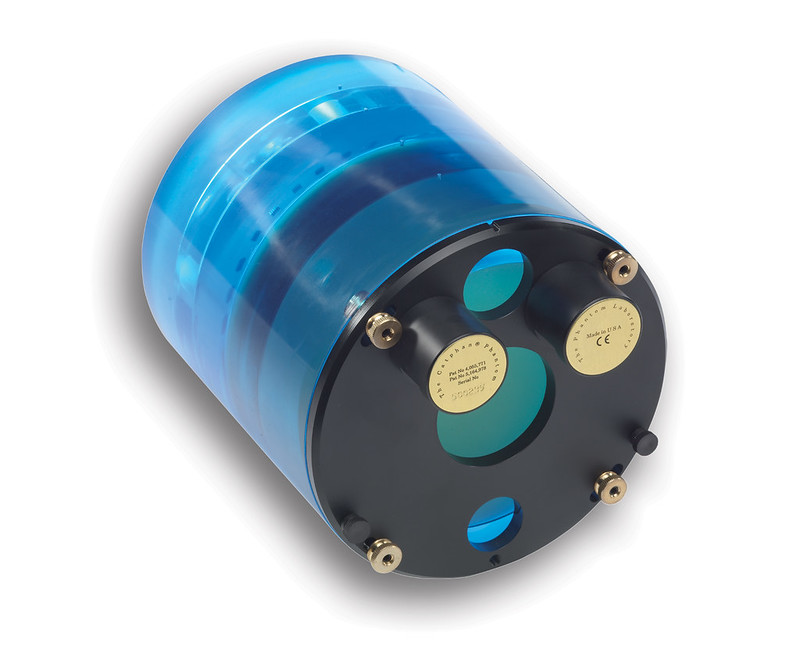
\includegraphics[width=0.3\textwidth]{Imagens/catphan1.jpg}
		}} %
        \subfigure{
		\fcolorbox{DarkTurquoise}{white}{%
			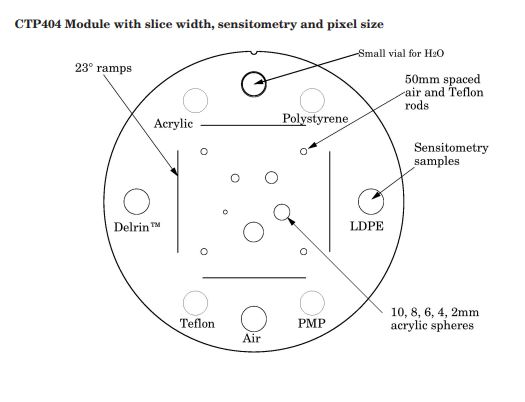
\includegraphics[width=0.3\textwidth]{Imagens/catphan2.JPG}
		}}%
        \subfigure{
		\fcolorbox{DarkTurquoise}{white}{%
			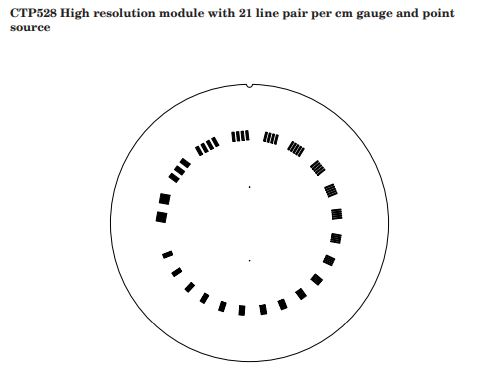
\includegraphics[width=0.3\textwidth]{Imagens/catphan3.JPG}
		}} \\ %
        \subfigure{
		\fcolorbox{DarkTurquoise}{white}{%
			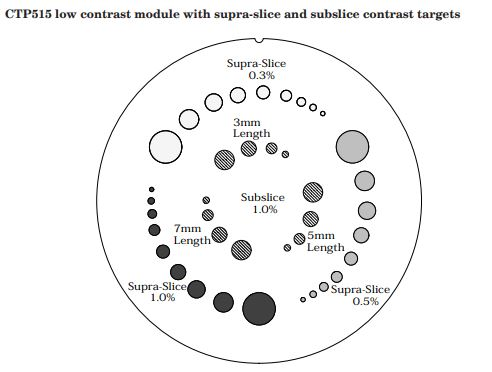
\includegraphics[width=0.3\textwidth]{Imagens/catphan4.JPG}
		}} %
        \subfigure{
		\fcolorbox{DarkTurquoise}{white}{%
			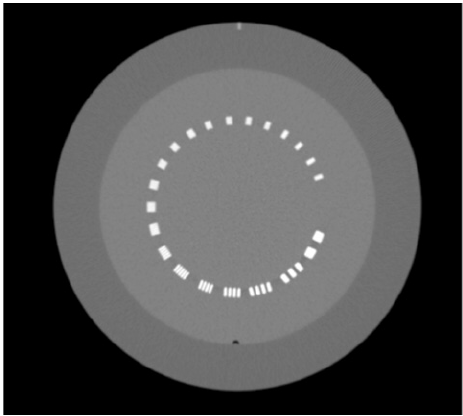
\includegraphics[width=0.25\textwidth]{Imagens/catphan5.png}
		}} %
        \subfigure{
		\fcolorbox{DarkTurquoise}{white}{%
			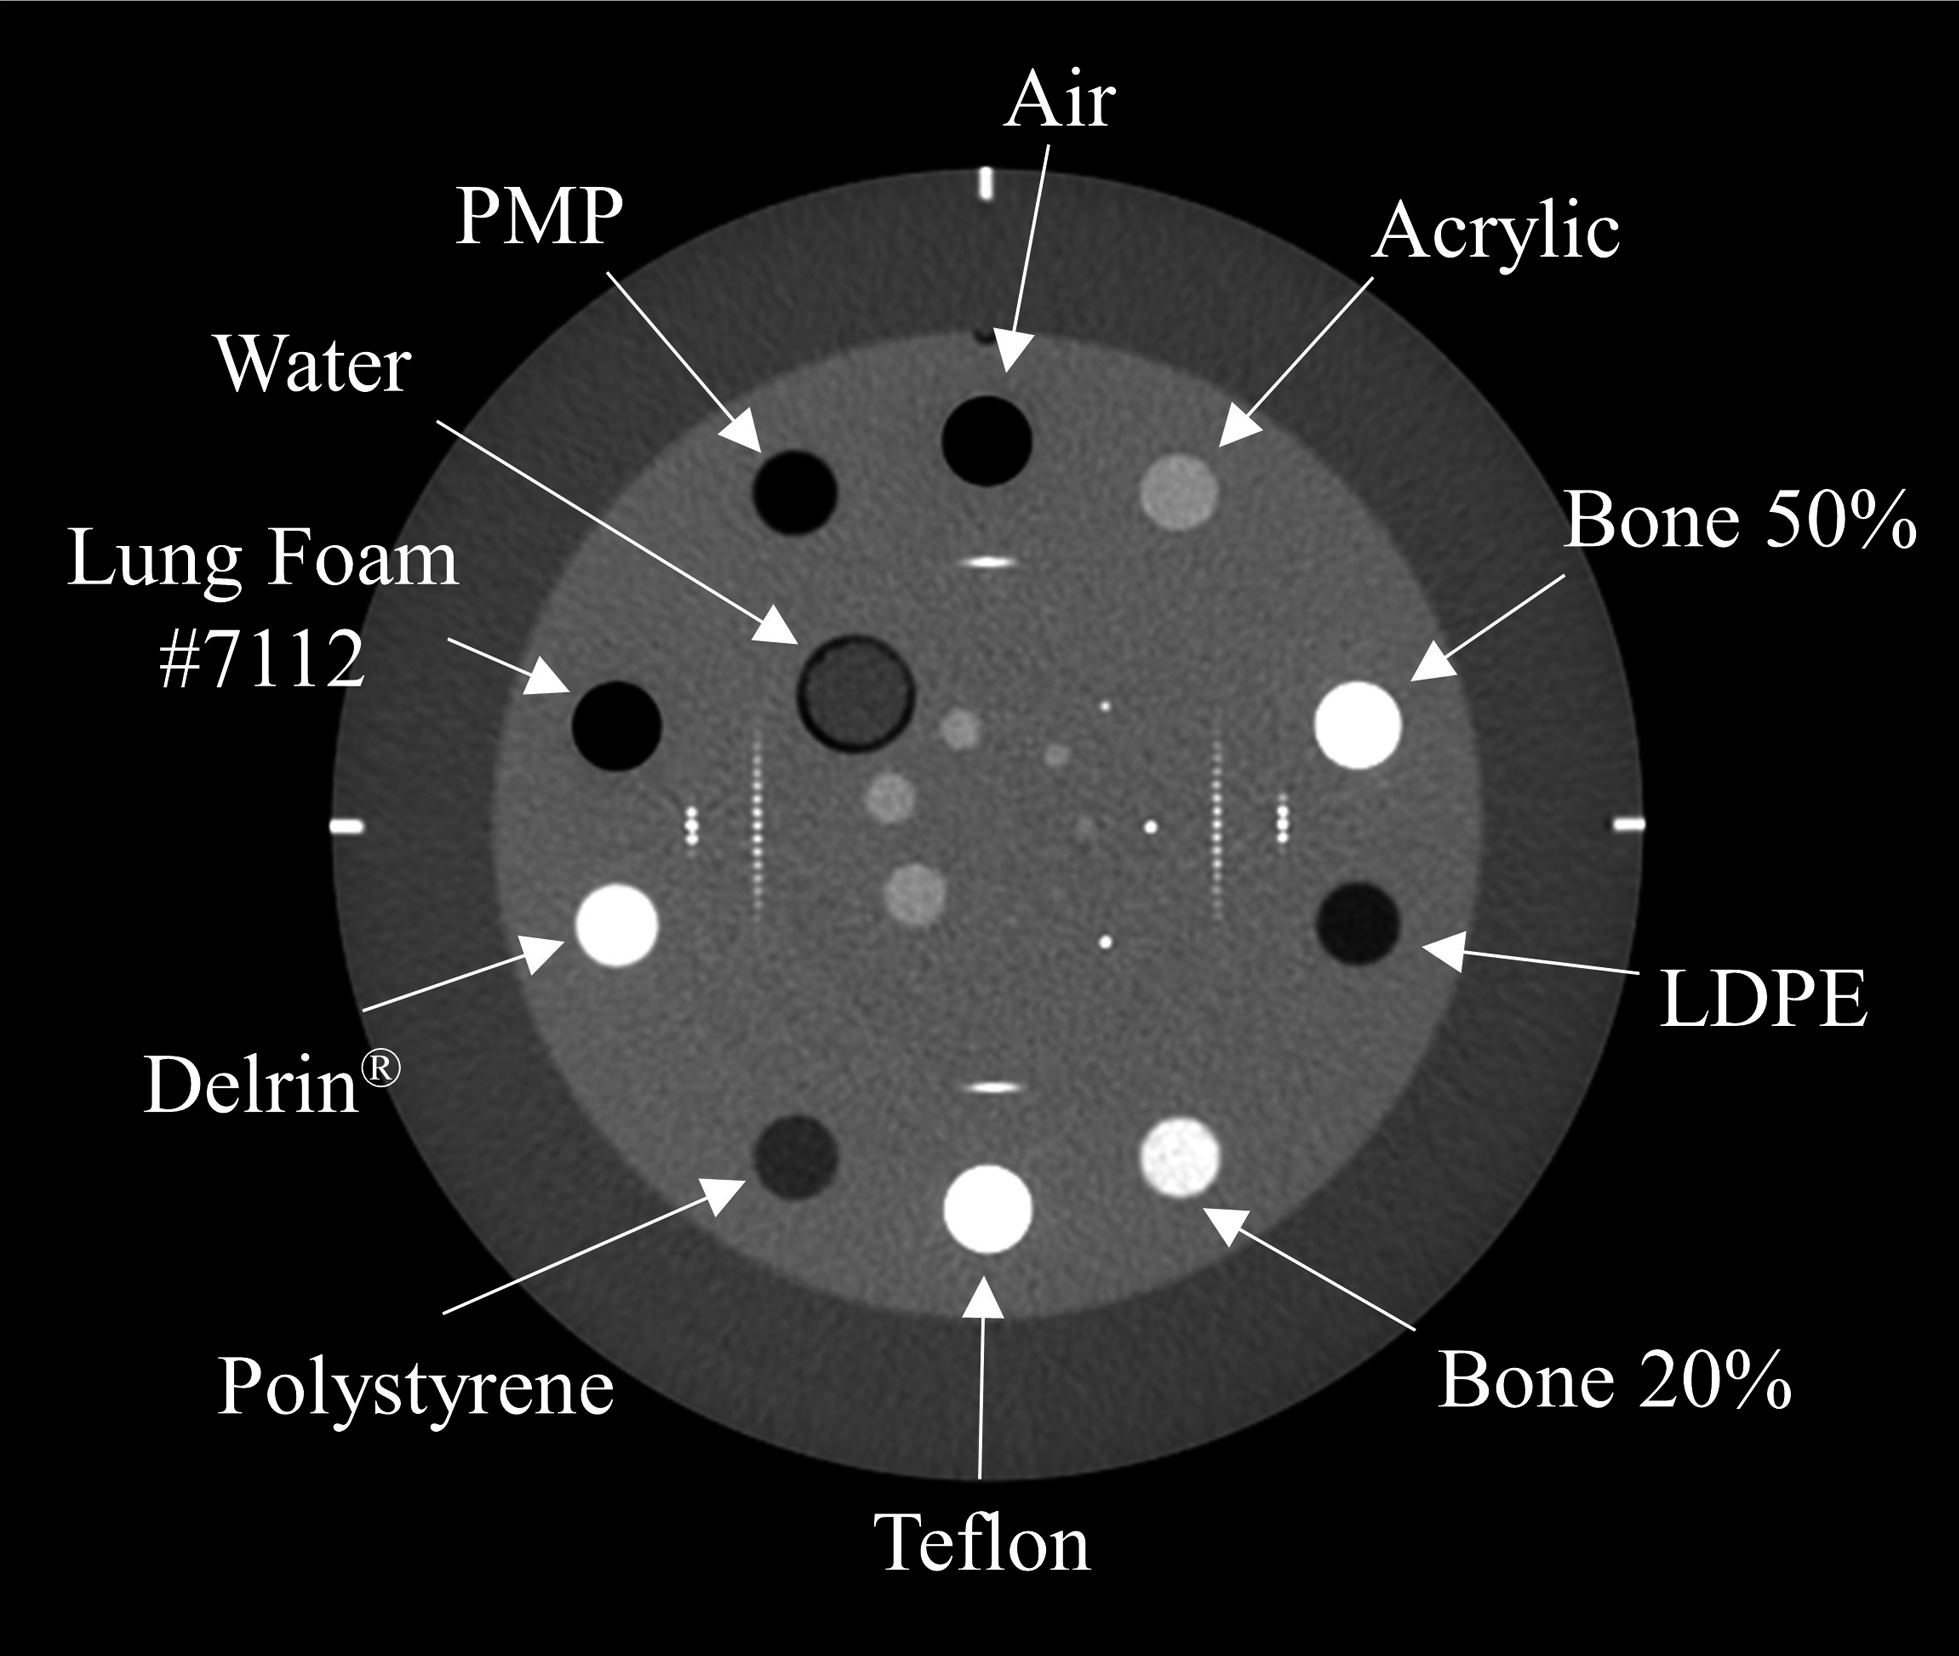
\includegraphics[width=0.3\textwidth]{Imagens/catphan6.jpg}
		}} %
        \caption{Phantom Catphan para QA de imagens de TC}
        \label{fig:catphan}
    \end{figure}




\subsection*{QA do Registro da Imagem (Fusão)}

    Um aspecto importante da cadeia de imagens é o registro de imagens (por exemplo, registro de uma ressonância magnética pré-tratamento com a de tomografia computadorizada de simulação para auxiliar no planejamento). O tópico de garantia de qualidade para registro de imagem é abordado no AAPM TG-132, \textit{``Use of Image Registration and Data Fusion Algorithms and Techniques in Radiotherapy Treatment Planning''}. QA é especialmente importante quando algoritmos automáticos são empregados.

\subsection*{Dose devido a Imagem}

    Como pode ser visto na \ref{fig:qaImagensParte2}, a maioria dos reports recomenda que a dose seja medida anualmente para as TCs adquiridas durante o tratamento e para imagens planares (kV ou MV). Portanto, é necessário que o físico médico saiba como fazer essas medidas. O AAPM TG-66 fornece orientação sobre a medida da dose devido a CT. A medida da dose de imagens planares kV é descrita no AAPM TG-2 (Relatório 39). A descrição dos princípios da dose absorvida medida pode ser encontrada no AAPM TG-7 de mamografia. Alguns centros consideram benéfico trabalhar com um físico do diagnóstico por imagem para medir a dose e avaliar os protocolos de imagem anualmente.

\subsection*{QA de Outros Sistemas de Localização}

    O QA de sistemas de localização não-radiográficos é discutido em AAPM TG-147. O AAPM TG-154 se concentra especificamente em sistemas de ultrassom utilizados em teleterapia. O TG-154 recomenda testes diários de alinhamento, testes mensais de phantom e laser offset, bem como controle de qualidade trimestral dos próprios phantoms de ultrassom, que estão sujeitos a dessecação. O controle de qualidade da qualidade da imagem é recomendado semestralmente e deve incluir resolução espacial, contraste e sensibilidade (ou seja, profundidade de penetração constante e ausência de artefatos). 
    
    Muitos sistemas não-radiográficos usam câmeras infravermelhas para localização dos pacientes, marcadores ou dispositivos. A precisão desses sistemas deve ser testada, pois estão sujeitos a possíveis efeitos de movimento e warm-up.

\subsection*{Recomendações de Testes, Frequências e Tolerâncias}

    A \ref{fig:qaImagensParte1} e a \ref{fig:qaImagensParte2} oferecem um guia com respeito à frequência com que os testes de QA devem ser realizados. Essas recomendações são baseadas em uma noção de quais erros seriam detectáveis em cada teste. Por exemplo, o AAPM TG-179 especifica testes diários de controle de qualidade projetados para “identificar quaisquer mudanças repentinas de desempenho ou erros grosseiros que possam resultar de colisões, atualizações ou serviço pós-horário”. Deve-se notar, no entanto, que os vários relatórios de grupo de tarefas e documentos de consenso não concordam sobre quais testes devem ser realizados ou sobre a frequência de tais testes.

    Para dar um exemplo, a frequência recomendada para testar a resolução espacial de um sistema CBCT varia de mensal (AAPM TG-142) a semestral (AAPM TG-179) e anualmente (AAPM TG-226). Outro exemplo são os testes de qualidade do feixe para CBCT. Isso é recomendado anualmente na AAPM TG-179, mas não tem recomendação específica na AAPM TG-142 ou AAPM TG-226. Alguns relatórios até parecem inconsistentes dentro de si mesmos. Por exemplo, o AAPM TG-142 recomenda um teste anual de qualidade do feixe para sistemas de imagem planar kV, mas não oferece tal recomendação para sistemas CBCT (embora um teste de constância do número de TC possa servir como um substituto). Os níveis de tolerância recomendados também diferem entre os relatórios e alguns relatórios defendem tolerâncias diferentes para algumas técnicas especializadas (por exemplo, stereotactic radiosurgery (SRS)/stereotactic body radiation therapy (SBRT)). 
    
    Parcialmente em uma tentativa de retificar essas divergências, a AAPM desenvolveu um documento de Diretriz de Prática de Física Médica (Medical Physics Practice Guideline - MPPG), o AAPM TG-226, \textit{``Commissioning and Quality Assurance of X-Ray Based Image-Guided Radiotherapy Systems''}. O AAPM TG-226 foi projetado para fornecer recomendações que são viáveis em um ambiente pequeno e com recursos limitados. Como tal, são diretrizes práticas mínimas. Como pode ser visto na \ref{fig:qaImagensParte1}, algumas das recomendações do AAPM TG-226 diferem substancialmente de outros relatórios do TG. 

\section{Resumo}

    Uma grande variedade de sistemas de aquisição de imagens estão disponíveis comercialmente que permitem imagens para orientação e localização durante o tratamento. Estes sistemas dependem de imagens radiográficas (por exemplo, imagens MV, imagens kV, kV CBCT e MV CT), imagens não radiográficas (por exemplo, US no quarto), imagens da superfície do paciente (por exemplo, marcadores de superfície reflexivos) e rastreamento do localização de marcadores implantados ou beacons eletromagnéticos. A chave para o uso eficaz desses sistemas IGRT é a compreensão e o controle do desempenho do sistema. Parâmetros relevantes incluem precisão geométrica, resolução espacial, contraste, ruído e uniformidade. Um programa estruturado de controle de qualidade é necessário para avaliar essas propriedades diariamente, mensalmente e anualmente. Os testes básicos de controle de qualidade são bem estabelecidos, embora haja algum desacordo nos relatórios da AAMP quanto ao tipo de teste e frequência. Um físico médico qualificado deve supervisionar o controle de qualidade, e os relatórios e resultados devem ser transparentes para a equipe, médicos e administradores. Uma questão final a considerar é a dose recebida pela imagem radiográfica. Embora as doses sejam muito mais baixas do que as doses terapêuticas (por exemplo, 1 a 3 cGy para uma varredura CBCT), os relatórios da AAMP sugerem que a dose de imagem deve ser considerada do ponto de vista de custo/benefício e minimizada na medida do possível.

\bibliography{ref.bib}
\end{document}